%% This is an example first chapter.  You should put chapter/appendix that you
%% write into a separate file, and add a line \include{yourfilename} to
%% main.tex, where `yourfilename.tex' is the name of the chapter/appendix file.
%% You can process specific files by typing their names in at the
%% \files=
%% prompt when you run the file main.tex through LaTeX.
\lstdefinestyle{codeStyle}{
language=C++,
    basicstyle=\footnotesize\ttfamily,
    keywordstyle=\color{blue}\ttfamily,
	keywordstyle=[2]\color{darkgreen},
    stringstyle=\color{red}\ttfamily,
    commentstyle=\color{green}\ttfamily,
    columns=flexible,
    gobble=4,
    frame=L,
    numbers=left,
    numberstyle=\tiny,
	%belowcaptionskip=2em,
    %belowskip=5em,
}

\lstdefinestyle{codeStyleFramed}{
language=C++,
    basicstyle=\footnotesize\ttfamily,
    keywordstyle=\color{blue}\ttfamily,
	keywordstyle=[2]\color{darkgreen},
    stringstyle=\color{red}\ttfamily,
    commentstyle=\color{green}\ttfamily,
    columns=flexible,
    gobble=4,
    frame=single,
    numbers=left,
    numberstyle=\tiny,
%	belowcaptionskip=2em,
 %   belowskip=5em,
}


\chapter{GPGPU - History And Motivation}


\section{Introduction}
GPGPU, acronym for General-purpose computing on graphics processing units, is a
recent phenomenon wich consist in the utilization of a graphics processing unit
(GPU\footnote{Graphic processing unit, term conied by Nvidia in the
mid-nineties, and now the most common acronym used.}), which typically handles
computation only for computer graphics and was optimized for a small set of
graphic operation, to perform computation in applications traditionally handled
by the central processing unit (CPU). Those operations (generation of 3D images)
are intrinsically parallel, so, is not surprising if the underlying hardware has
evolved into a highly parallel, multithreaded, and many-core processor. The GPU excels at fine grained,
data-parallel workloads consisting of thousands of independent threads executing vertex,
geometry, and pixel-shader program threads concurrently.
Nowadays, the GPUs are not limited to its use as a graphics engine; there is a rapidly
growing interest in using these units as parallel computing architecture due to the tremendous
performance available in them. Currently, GPUs outperform CPUs on floating
point performance and memory bandwidth, both by a factor of roughly
100\cite{NvidiaprogGuide}, easily reaching computational powers in the
order of teraFLOPS. GPU works alongside the CPU providing an heterogeneous
computation, simply offloading compute-data-intensive portion of program on GPU
using it as co-processor highly specialized in parallel tasks.
Plus since 2006, date when Nvidia has introduced CUDA, is extremely simple to
program these kind of devices for general purpose tasks, although before that
date this goal was achieved dealing directly with the graphic API using shaders
with all the related constraints such as lack of integers or bit operations.



\section{Why GPU computing?}
Traditionally performance improvements in computer architecture have come from
cramming ever more functional units onto silicon, increasing clock speeds and
transistors number. Moores law\cite{mooreLaw1965} states that the number of
transistors that can be placed inexpensively on an integrated circuit will
double approximately every two years.
\begin{figure}
\centering
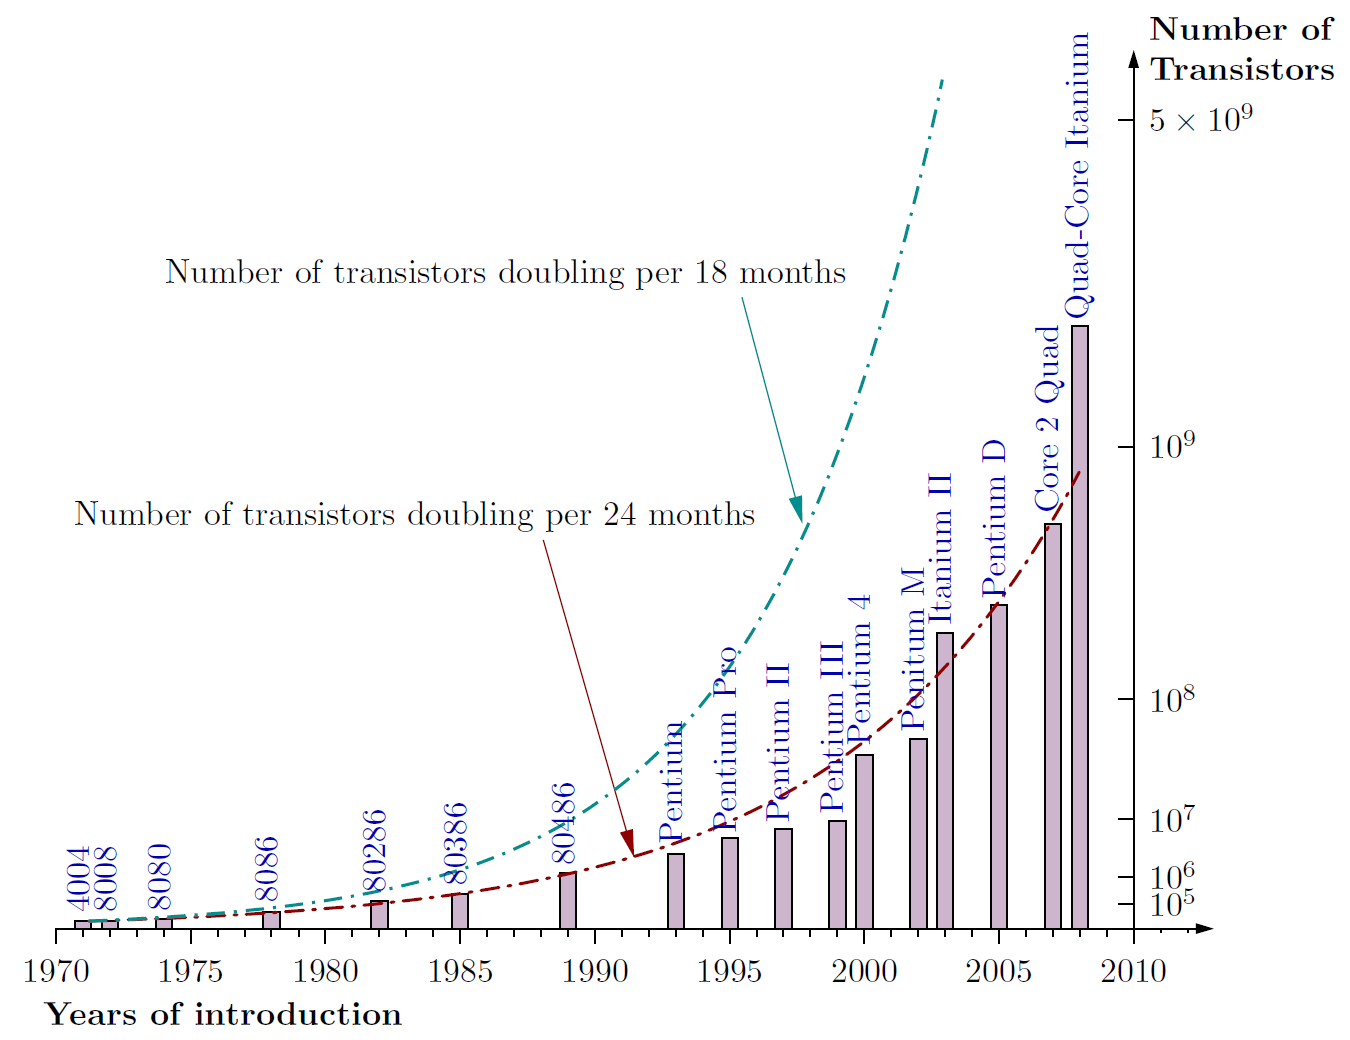
\includegraphics[totalheight=0.5\textheight]{./images/moore_law_large}
\caption{Moore's Law and intel family CPU transistors number
history.}\label{mooreLaw}
\end{figure}

Coupled with increasing clock speeds CPU performance has until recently scaled
likewise. But this trend cannot be sustained indefinitely or forever.
Increased clock speed and transistor number require more power and generate more
heat. Although the trend for transistor densities has continued to steadily increase,
clock speeds began slowing circa 2003 at 3 GHz. If we apply Moore's law type
thinking to clock-speed performance, we should be able to buy at least 10 GHz CPUs. However, the fastest CPU available today is 3.80 GHz 
At same point the performance increase fails to increase proportionally
with the added effort in terms of transistors or clock speed because efficient
heat dissipation and increasing transistor resolution on a wafer becomes more
important and challenging (there will be still the physical limit of dimension
for each transistor, the atom).
The heat emitted from the modern processor, measured in power
density	\begin{math}(\frac{W}{cm^2})\end{math} rivals
the heat of a nuclear reactor core\cite{Gelsinger2004}.
\begin{figure}[h!]
\centering
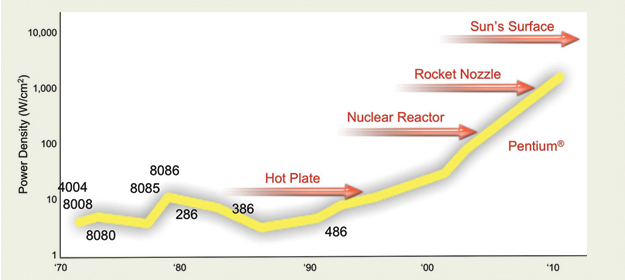
\includegraphics[scale=0.7]{./images/temperatureCPU}
\caption{Temperature CPUs}\label{tempCPU}
\end{figure}
But the power demand did not stop in these year, here the necessity of
switching on parallel architectures, so today the dominating trend in commodity CPU
architectures is multiple processing cores mounted on a single die operating at
reduced clock speeds and sharing some resources. Today is normal to use the so-called
multi-core (2,4,8,12) CPUs on a desktop PC at home.



\section{From Graphics to General Purpose Computing}
The concept of many processor working together in concert in not new in the
graphic field of the computer science. Since the demand generated by
entertainment started to growth multi-core hardware emerged in
order to take advantage of the high parallel task of generating 3D image.
In computer graphics, the process of generating a 3D images consist of
refreshing pixels at rate of sixty or more Hz. Each pixel to be processed
goes through a number of stages, and this process is commonly referred to as
the graphic processing pipeline. The peculiarity of this task is that the
computation each pixel is independent of the other's so this work is perfectly
suitable for distribution over parallel processing elements.
To support extremely fast processing of large graphics data sets (vertices and fragments), modern GPUs employ a
stream processing model with parallelism.
The game industry boosted the development of the GPU, that offer now greater
performance than CPUs and are improving faster too (see Figure
\ref{CPU-VS-GPU_GFLOP} and \ref{CPU-VS-GPU_MEMORY}).
The reason behind the discrepancy in floating-point capability between CPU and
GPU is that GPU is designed such that more transistors are devoted to data
processing rather than caching and flow control.

The today's Top 500 Supercomputers\footnote{\url{http://www.top500.org/statistics/list/}} ranking is
dominated by massively parallel computer, built on top of superfast networks and millions of
sequential CPUs working in concert but as the industry is developing even more
powerful, programmable and capable GPUs in term of GFlops  we see
that they begin to offer advantages over traditional cluster of computers in
terms of economicity and scalability.

\begin{figure}
\centering
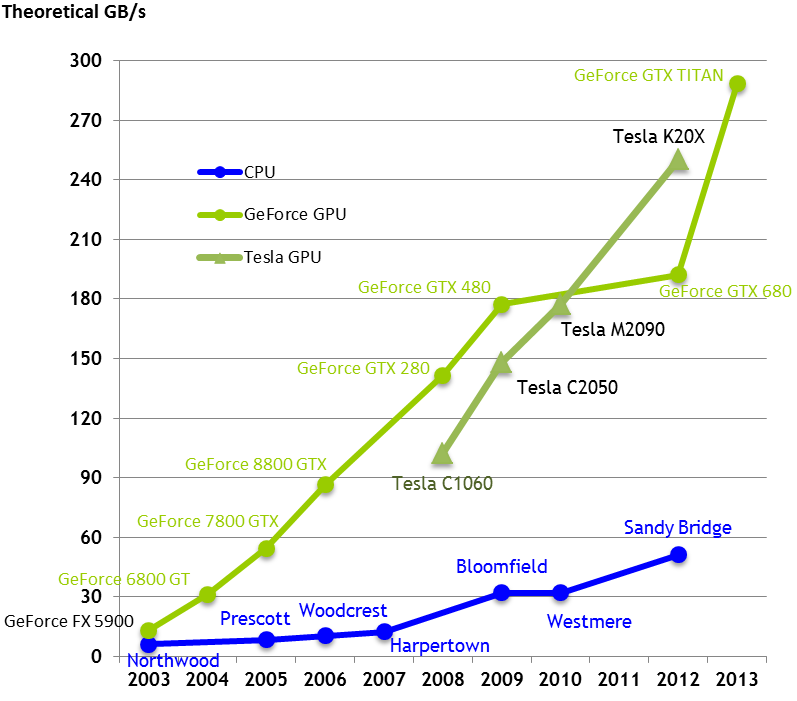
\includegraphics[scale=0.4]{./images/memory-bandwidth}
\caption{Intel CPUs and Nvidia GPUs memory bandwidth
chart}\label{CPU-VS-GPU_MEMORY}
\end{figure}
\begin{figure}
\centering
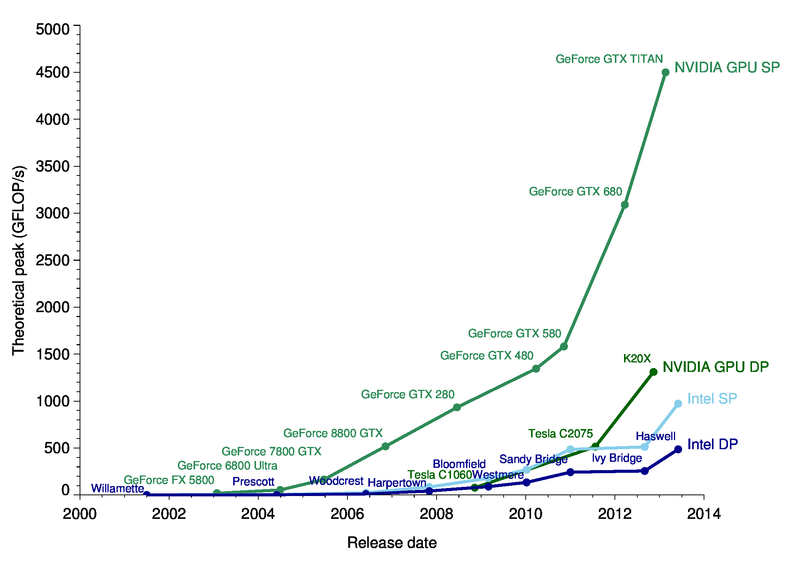
\includegraphics[scale=0.4]{./images/cpu-vs-gpu}
\caption[Intel CPUs and Nvidia GPUs Peak G/FLOPS chart]{Intel CPUs and Nvidia
GPUs (single and double precision) Peak G/FLOPS chart}\label{CPU-VS-GPU_GFLOP}
\end{figure}


\subsection{Traditional Graphics Pipeline}\label{graphicPipeline}
A graphics task such as rendering a 3D scene on the GPU
involves a sequence of processing stages (i.e. shaders) that run in parallel
and in a prefixed order, known as the graphics hardware
pipeline\footnote{http://duriansoftware.com/joe/An-intro-to-modern-OpenGL.-Chapter-1:-The-Graphics-Pipeline.html}
(see Figure \ref{graphicPipeline}).


The first stage of the pipeline is the vertex processing. The
input to this stage is a 3D polygonal mesh. The 3D world coordinates of each vertex of the mesh
are transformed to a 2D screen position. Color and texture
coordinates associated with each vertex are also evaluated.
In the second stage, the transformed vertices are grouped
into rendering primitives, such as triangles. Each primitive
is scan-converted, generating a set of fragments in screen
space. Each fragment stores the state information needed
to update a pixel. In the third stage, called the fragment processing, the texture coordinates of each fragment are used
to fetch colors of the appropriate texels (texture pixels) from
one or more textures. Mathematical operations may also be
performed to determine the ultimate color for the fragment.
Finally, various tests (e.g., depth and alpha) are conducted to
determine whether the fragment should be used to update a
pixel in the frame buffer.
Each shader in the pipeline performs a basic but specialised operation on the
vertices as it passes.
In a shader based architecture the individual shader processors exhibit very limited
capabilities beyond their specific purpose.
Before the advent of CUDA in 2006 most of the techniques for non-graphics
computation on the GPU took advantages of the programmable fragment processing
stage. The steps involved in mapping a computation on the GPU are
as follows:
\begin{figure}
\centering
\caption{Typical graphic pipeline}\label{graphicPipeline}
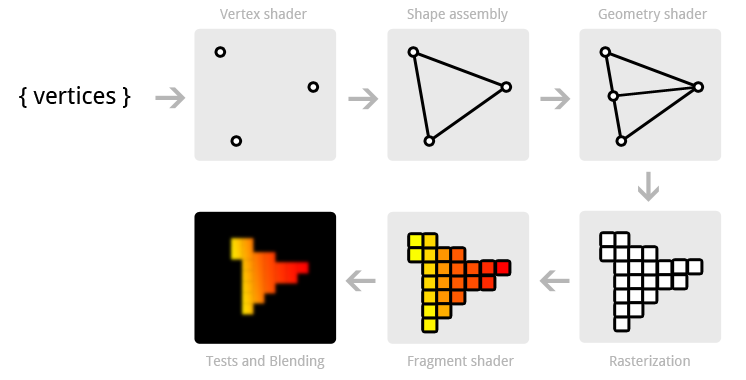
\includegraphics[scale=0.6]{./images/pipeline}
\end{figure}

\begin{enumerate}
	\item The data are laid out as texel colors in textures;
	\item  Each computation step is implemented with a
			user-defined fragment program. The results are encoded as pixel 
			colors and rendered into a pixel-buffer\footnote{ A buffer in GPU memory
			which is similar to a frame-buffer.}; 
	\item Results that are
			to be used in subsequent calculations are copied to textures for temporary
		storage.
\end{enumerate} 

The year 2006 marked a significant turning point in GPU architecture. The G80
was the first NVidia GPU to have a unified architecture whereby the different shader processors were
combined into unified stream processors. The resulting stream processors had to be
more complex so as to provide all of the functionality of the shader processors they
replaced. Although research had been carried out into general purpose programming
for GPUs previously, this architectural change opened the door to a far wider range of
applications and practitioners.
More in detail GPU are well-suited for problems highly data-parallel in wich the
same code is executed on many data elements at the same time (SIMD
paradigm\footnote{Single Instruction,
Multiple Data:
elements of short vectors are processed in parallel. To be clear CUDA paradigm is SIMT: Single
Instruction, Multiple Threads} or more generally as a CRCW PRAM
machine\footnote{Parallel random-access machine in which each thread can read
or write a memory cell.}).








